\documentclass[tikz,border=6pt]{standalone}
\usepackage{tikz}
\usetikzlibrary{patterns,arrows.meta,calc,decorations.markings,positioning}
\begin{document}
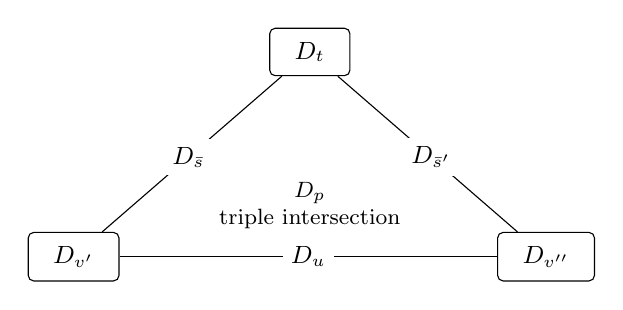
\begin{tikzpicture}[font=\small,
    diagramrange/.style={draw,rounded corners=2pt,fill=white,
                  inner xsep=9pt,inner ysep=5pt},
    overlap/.style={fill=white,inner sep=3pt}]
  \node[diagramrange] (t) at (0,1.8) {$D_t$};
  \node[diagramrange] (v) at (-3,-.8) {$D_{v'}$};
  \node[diagramrange] (w) at (3,-.8) {$D_{v''}$};
  \draw (t) -- node[overlap,pos=.52] {$D_{\bar s}$} (v);
  \draw (t) -- node[overlap,pos=.52] {$D_{\bar s'}$} (w);
  \draw (v) -- node[overlap] {$D_u$} (w);
  \node[align=center,font=\footnotesize] at (0,-.15)
    {$D_p$\\triple intersection};
\end{tikzpicture}
\end{document}
